\documentclass{article}

\usepackage{tikz}
\usetikzlibrary{automata, positioning, arrows}

\tikzset{
    ->,
    node distance=3cm,
    every state/.style={thick, fill=gray!10},
    initial text=$ $,
}

\begin{document}

\begin{figure}[ht]
    \centering
    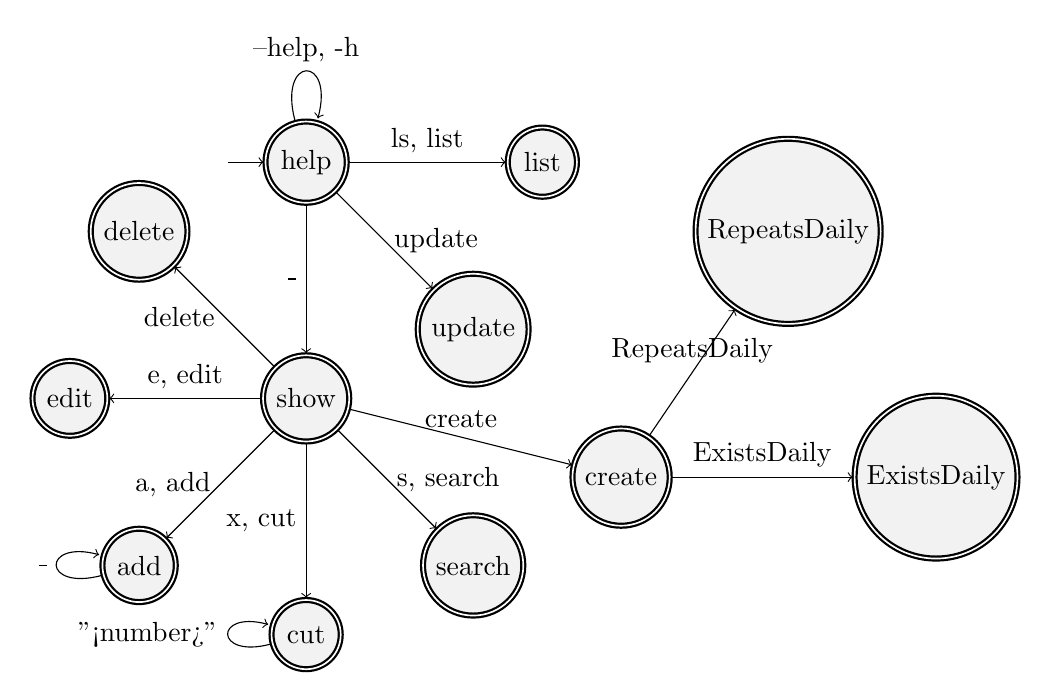
\begin{tikzpicture}
        \node[state, initial, accepting] (help) {help};
        \node[state, accepting, right of=help] (list) {list};
        \node[state, accepting, below right of=help] (update) {update};
        \node[state, accepting, below of=help] (show) {show};
        \node[state, accepting, right of=show, xshift=1cm, yshift=-1cm] (create) {create};
        \node[state, accepting, above right of=create, yshift=1cm] (RepeatsDaily) {RepeatsDaily};
        \node[state, accepting, right of=create, xshift=1cm] (ExistsDaily) {ExistsDaily};
        \node[state, accepting, left of=show] (edit) {edit};
        \node[state, accepting, below left of=show] (add) {add};
        \node[state, accepting, below of=show] (cut) {cut};
        \node[state, accepting, below right of=show] (search) {search};
        \node[state, accepting, above left of=show] (delete) {delete};

        \draw (help) edge[loop above] node{--help, -h} (help)
              (help) edge[above] node{ls, list} (list)
              (help) edge[right] node{update} (update)
              (help) edge[left] node{\_} (show)
              (show) edge[above] node{create} (create)
              (create) edge[above] node{RepeatsDaily} (RepeatsDaily)
              (create) edge[above] node{ExistsDaily} (ExistsDaily)
              (show) edge[above] node{e, edit} (edit)
              (show) edge[left] node{a, add} (add)
              (add) edge[loop left] node{\_} (add)
              (show) edge[left] node{x, cut} (cut)
              (cut) edge[loop left] node{"<number>"} (cut)
              (show) edge[right] node{s, search} (search)
              (show) edge[left] node{delete} (delete)
              ;
    \end{tikzpicture}
\end{figure}

\end{document}
